\documentclass[a4paper,12pt]{article}
\usepackage[left=3cm, right=3cm, top=3cm, bottom=3cm,margin=3cm]{geometry}
\usepackage{enumitem}
\usepackage{amsmath}
\usepackage{amssymb}
\usepackage{physics}
\usepackage{multicol}
\usepackage{graphicx}
\usepackage{titling}
\usepackage{graphicx}
\usepackage{color,xcolor}
\usepackage{tikz}
\usepackage{tikz-3dplot}
\usepackage{wrapfig}
\usepackage{pgfplots, tkz-euclide,calc}
    \usetikzlibrary{patterns,snakes,shapes.arrows,3d}
    \usepgfplotslibrary{fillbetween}

\newcommand{\del}{\partial}

\pgfplotsset{compat=1.18}

\title{\textbf{Tugas Analisis Vektor} 
\vspace{0.5cm}
\\ \large \textbf{Pembahasan Soal Bu Nur}}

%\author{Renaldy Satriaji Wahyudi}
\date{}
\pagestyle{empty}

\begin{document}

\begin{titlepage}

\maketitle
\thispagestyle{empty}

\begin{figure}[h]
    \centering
    \includegraphics[width=0.5\linewidth]{logoITS.png}
\end{figure}

\begin{center}
\textbf{Anggota Kelompok 10}
\end{center}
\begin{enumerate}
    \item Nicholas Joe Sumantri \hfill (5002221003)
    \item Renaldy Satriaji  Wahyudi \hfill (5002221155)
    \item Teosofi Hidayah Agung \hfill (5002221132)
    \item Bagus Rico Pambudi \hfill (5002221144)
\end{enumerate}

\begin{tikzpicture}[remember picture, overlay]
        \node[anchor=south, yshift=4cm] at (current page.south) {
            \begin{minipage}{\textwidth}
                \centering
                \textbf{Departemen Matematika}\\
                \textbf{Institut Teknologi Sepuluh Nopember}\\
                \textbf{Semester Genap 2023/2024}
            \end{minipage}
        };
    \end{tikzpicture}
\end{titlepage}



\newpage

\section*{SOAL \& PEMBAHASAN  }
\begin{enumerate}
    \item \textbf{[SOAL]}\\
          Diketahui fungsi vektor \( \vec{F}(x,y) = 2xy^3 \hat{i} + (1 + 3xy^2) \hat{j} \)
        \begin{enumerate}[start = 1]
         \item  Buktikan bahwa \( \vec{F}(x,y) \) adalah medan vektor konservatif pada bidang-$xy$.
         \( \vec{F} \) dikatakan medan vektor konservatif saat \( \nabla \times \vec{F} = 0 \).
         
         \item Jika gaya \( \vec{F}(x,y) \) adalah konservatif maka \( \vec{F} = \nabla \phi \) dan \( \phi (x,y) \) disebut potensial \( \vec{F} = \nabla \phi \).
         
\end{enumerate}

        \textbf{[PEMBAHASAN]}
        \begin{enumerate}[start = 1]
        \item \[
            \nabla \times \vec{F} = \begin{vmatrix}
            \hat{i} & \hat{j} & \hat{k} \\
            \frac{\partial}{\partial x} & \frac{\partial}{\partial y} & \frac{\partial}{\partial z} \\
            2xy^3 & 1 + 3xy^2 & 0
            \end{vmatrix}
            = \hat{i} (0 - 0) - \hat{j} (0 - 0) + \hat{k} (6xy^2 - 6xy^2) = 0
            \]
        \item \[
2xy^3 \hat{i} + (1 + 3x^2y^2) \hat{j} = \left(\frac{\partial \phi}{\partial x} \hat{i} + \frac{\partial \phi}{\partial y} \hat{j} + \frac{\partial \phi}{\partial z} \hat{k} \right)
\]

\vspace{0.2cm}

\begin{itemize}
    \item
    \[
    \frac{\partial \phi}{\partial x} = 2xy^3
    \]
        
    \[
    \int {\partial \phi}  = \int 2xy^3 \, dx
    \]
        
    \[
    \phi = x^2y^3 + f(y)
    \]
\end{itemize}

\vspace{0.5cm}

\begin{itemize}
\item
        \[\frac{\partial \phi}{\partial y} = 3x^2y^2 + f'(y)\]
        
        \[1 + 3x^2y^2 = 3x^2y^2 + f'(y)\]
        
        \[f'(y) = 1\]
        
        \[f(y) = y\]
        
\end{itemize}

\vspace{0.5cm}

\textbf{maka :\hspace{4cm}} \fbox{\(\phi = x^2y^3 + y\)}

 \end{enumerate}

\newpage
    \item \textbf{[SOAL]}\\
        Diberikan $\displaystyle I = \oint_{C} (x - y)\, dx + (x + y)\, dy$. Jika $C$ kurva tertutup yang membatasi daerah $y = x^{3}$ dan $x=y^{2}$
            \begin{enumerate}[start = 1]
                \item Hitung integral tersebut tanpa menggunakan teorema Green.
                \item Hitung integral tersebut dengan menggunakan teorema Green.
            \end{enumerate}

        \textbf{[PEMBAHASAN]}
        \begin{itemize}
            \item $\displaystyle I = \oint_{C} (x - y)\, dx + (x + y)\, dy$
            \item $C$ kurva tertutup yang membatasi daerah $y = x^{3}$ dan $x = y^{2}$
        \end{itemize}
        \begin{enumerate}[start = 1]
            \item Hitung integral tersebut tanpa menggunakan teorema green

        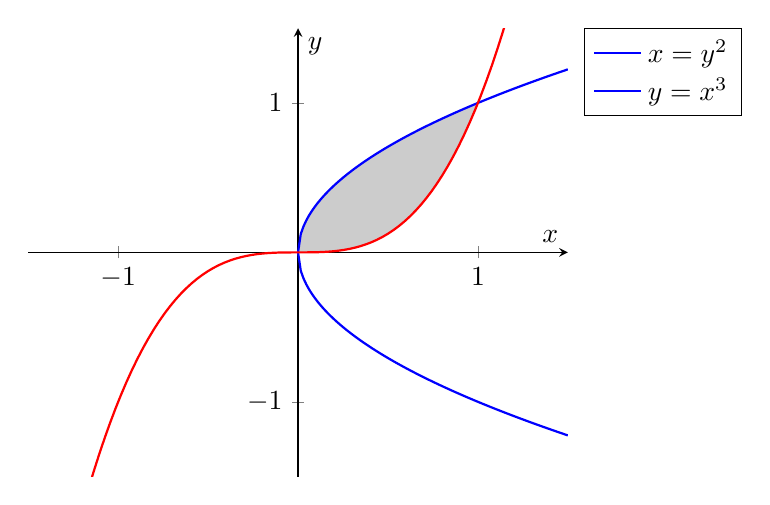
\begin{tikzpicture} %Gambar grafik batas daerah
            \begin{axis}[
                axis lines = middle,
                xtick = {-1,0,1},
                xlabel = {$x$},
                ylabel = {$y$},
                xmin=-1.5, xmax=1.5,
                ymin=-1.5, ymax=1.5,
                domain=-1.5:1.5,
                samples=100,
                legend pos=outer north east
                ]
                % Plot x = y^2 (rewritten as y = sqrt(x) and y = -sqrt(x))
                \addplot [
                domain=0:1.5,
                samples=100,
                color=blue,
                thick,
                name path=A
                ] {sqrt(x)};
                \addlegendentry{$x = y^2$}
    
                \addplot [
                domain=0:1.5,
                samples=100,
                color=blue,
                thick
                ] {-sqrt(x)};
    
                % Plot y = x^3
                \addplot [
                domain=-1.5:1.5,
                samples=100,
                color=red,
                thick,
                name path=B
                ] {x^3};
                \addlegendentry{$y = x^3$}
                
                \addplot[fill=gray,opacity=0.4] fill between[of=A and B,split,soft clip={domain=0:1}];
            \end{axis}
        \end{tikzpicture}

        \begin{itemize}
            \item $\mathbf{y = x^{3}}$\\
                $x = t,\ dx = dt$\\
                $y = t^{3},\ dy = 3t^{2}$
        \end{itemize}

        \begin{align*}
            \int_{0}^{1} (t - t^{3})\, dt + (t +t^{3}) 3t^{2}\, dt & = \int_{0}^{1} t + 2t^{3} +3t^{5}\, dt\\
            & = \dfrac{1}{2} t^{2} + \dfrac{1}{2} t^{4} + \dfrac{1}{2} t^{6}\ \bigg|_{0}^{1}\\
            & = \dfrac{1}{2} + \dfrac{1}{2} + \dfrac{1}{2}\\
            & = \mathbf{\dfrac{3}{2}}
        \end{align*}

\newpage

        \begin{itemize}
            \item $\mathbf{x = y^{2}}$\\
                $x = t^{2},\ dx = 2t\, dt$\\
                $y = t,\ dy = dt$
        \end{itemize}

        \begin{align*}
            \int_{1}^{0} (t^{3} - t) 2t\, dt + (t^{2} + t)\, dt & = \int_{1}^{0} 2t^{3} - t^{2} + t\, dt\\
            & = \dfrac{1}{2} t^{4} - \dfrac{1}{3} t^{3} + \dfrac{1}{2} t^{2}\ \bigg|_{1}^{0}\\
            & = \left(\dfrac{1}{2} - \dfrac{1}{3} + \dfrac{1}{2}\right)\bigg|_{1}^{0}\\
            & = -\dfrac{1}{2} + \dfrac{1}{3} - \dfrac{1}{2}\\
            & = \mathbf{-\dfrac{2}{3}}
        \end{align*}

        \textbf{Hasil :} $\mathbf{\dfrac{3}{2} + \left(-\dfrac{2}{3}\right) = \dfrac{5}{6}}$

        \item Hitung integral tersebut dengan menggunakan teorema Green.

        \begin{align*}
        \oint_{C} M\, dx + N\, dy & = \iint_{R} \dfrac{\partial{N}}{\partial{x}} - \dfrac{\partial{M}}{\partial{y}}\, dx\ dy\\
        \oint_{C} (x - y)\, dx + (x + y)\, dy & = \iint_{R} 1 - (-1)\, dx\ dy = \iint_{R} 2\, dx\ dy\\
        & = \int_{x = 0}^{1} \int_{y = x}^{\sqrt{x}} 2\, dx\ dy = \int_{x = 0}^{1} 2y\ \bigg|_{x^{3}}^{\sqrt{x}}\, dx\\
        & = \int_{x = 0}^{1} 2\sqrt{x} - 2x^{3}\, dx  = 2 \left(\dfrac{2}{3} x^{\frac{3}{2}} - \dfrac{1}{4} x^{4}\right)\ \bigg|_{0}^{1}\\
        & = 2\left(\dfrac{2}{3} - \dfrac{1}{4}\right) = 2\left(\dfrac{8 - 3}{12}\right)\\
        & = \mathbf{\dfrac{5}{6}}
        \end{align*}

        \textbf{Hasil :} $\mathbf{\dfrac{5}{6}}$
        
    \end{enumerate}
    \item \textbf{[SOAL]}\\
    Gunakan teorema Stokes untuk menghitung $\displaystyle\oint_C \vb*{F} \cdot d\vb*{r}$ dengan $\vb*{F}=xy\vb*{i} + yz\vb*{j} + zx\vb*{k}$ dan $C$ adalah segitiga dengan titik sudut $(1,0,0),\,(0,1,0),\,(0,0,1)$ terorientasikan searah dengan putaran jarum jam bila dilihat dari atas.

    \textbf{[PEMBAHASAN]}\\
    \begin{center}
        \tdplotsetmaincoords{60}{110}
        \begin{tikzpicture}[tdplot_main_coords,scale=2]
        \pgfmathsetmacro{\step}{0.01}
        %%% Coordinate axis
        \draw[thick,->] (0,0,0) -- (1.5,0,0) node [below left] {\footnotesize$x$};
        \draw[dashed] (0,0,0) -- (-0.5,0,0);
        \draw[thick,->] (0,0,0) -- (0,1.5,0) node [right] {\footnotesize$y$};
        \draw[dashed] (0,0,0) -- (0,-0.5,0);
        \draw[thick,->] (0,0,0.0) -- (0,0,1.5) node [above] {\footnotesize$z$};
        % The curves slicing the surface
        \draw[blue,fill=cyan,very thick,opacity=0.5] (1,0,0) -- (0,1,0) -- (0,0,1)--cycle;
        \foreach \x in {1} 
        \draw[shift={(\x,0,0)},color=black] (0pt,0.01pt,0pt) -- (0pt,-0.01pt,0pt) node[left] {$\x$};
        \foreach \x in {1} 
        \draw[shift={(0,\x,0)},color=black] (0.01pt,0pt,0pt) -- (-0.01pt,0pt,0pt) node[above] {$\x$};
        \end{tikzpicture}
    \end{center}
    Teorema Stokes menyatakan bahwa $\displaystyle\oint_C \vb*{F} \cdot d\vb*{r} = \iint_S (\curl \vb*{F}) \cdot n\,dS$.
        \begin{flalign*}
        \curl \vb*{F} = \begin{vmatrix}
            \vb*{i} & \vb*{j} & \vb*{k}\\
            \del_x & \del_y & \del_z\\
            xy & yz & zx
        \end{vmatrix} = (0-y)\vb*{i} - (z-0)\vb*{j} + (0-x)\vb*{k} = -y\vb*{i} - z\vb*{j} - x\vb*{k}
        \end{flalign*}
        Persamaan bidang $S$ adalah $x+y+z=1$. Normal vektor bidang $S$ adalah $\vb*{n} = \vb*{i} + \vb*{j} + \vb*{k}$. Sehingga
        \begin{flalign*}
            dS=\frac{\vb*{n}}{\norm{\vb*{n}}}dA = \frac{1}{\sqrt{3}}(\vb*{i} + \vb*{j} + \vb*{k})dA
        \end{flalign*}
        Kemudian akhirnya didapatkan
        \begin{flalign*}
            \iint_S (\curl \vb*{F}) \cdot n\,dS &= \iint_S (-y\vb*{i} - z\vb*{j} - x\vb*{k}) \cdot (\vb*{i} + \vb*{j} + \vb*{k})\frac{1}{\sqrt{3}}dA&\\
            &= \frac{1}{\sqrt{3}}\iint_S (-y-z-x)dA&\\
            &= \frac{1}{\sqrt{3}}\int_0^1\int_0^{1-x}\left(-x-y-(1-x-y)\right)dydx&\\
            &= \frac{1}{\sqrt{3}}\int_0^1\int_0^{1-x}(-1)dydx&\\
            &= \frac{-1}{\sqrt{3}}\int_0^1 1-x\,dx&\\
            &= \frac{1}{\sqrt{3}}\int_0^1 x-1\,dx&\\
            &= \frac{1}{\sqrt{3}}\left(\frac{x^2}{2}-x\right)\Big|_0^1&\\
            &= \frac{1}{\sqrt{3}}\left(\frac{1}{2}-1\right)=-\frac{1}{2\sqrt{3}}
        \end{flalign*}
    

    \item \textbf{[SOAL]}\\
    Hitung fluks medan vektor $\displaystyle\iint_S \vb*{F} \cdot n\,dS$ jika diberikan vektor gaya $\vb*{F} = 4x\vb*{i} + 2y^2\vb*{j} + z^2\vb*{k}$ menembus permukaan tertutup $S$ yang dibatasi oleh $x^2 + y^2 = 4$ dan $z=3$.
        
        \textbf{[PEMBAHASAN]}
        \begin{itemize}
    \item Dengan Teorema Gauss
    \[
    \iint_S \vec{F} \cdot \vec{n} \, dS = \iiint_V (\nabla \cdot \vec{F}) \, dV.
    \]

    \item Divergensi $\vec{F}$:
    \[
    \nabla \cdot \vec{F} = \frac{\partial}{\partial x} (4x) + \frac{\partial}{\partial y} (-2y^2) + \frac{\partial}{\partial z} (z^2).
    \]
    \[
    = 4 - 4y + 2z.
    \]

    \item Integral volume:
    \[
    V \text{ dibatasi } x^2 + y^2 = 4 \rightarrow r = 2, \, z = 0 \, \text{ sampai } \, z = 3. \text{ Ubah ke koordinat kutub.}\]
    \begin{flalign*}
    \iiint_V (4 - 4y + 2z) \, dV &= \iiint_V (4 - 4(r \sin \theta + 2z) \, r \, dr \, d\theta \, dz&\\
    &= \int_0^3 \int_0^{2\pi} \int_0^2 (4r - 4r^2 \sin \theta + 2zr) \, dr \, d\theta \, dz&\\
    &= \int_0^3 \int_0^{2\pi} \left[ 2r^2 - \frac{4r^3 \sin \theta}{3} + 2r^2 \right]_0^2 \, d\theta \, dz&\\
    &= \int_0^3 \int_0^{2\pi} \left[ 8 - \frac{32}{3} \sin \theta + 4z \right] \, d\theta \, dz&\\
    &= \int_0^3 \left[ 16\pi + \frac{32}{3} \cos \theta + 4z \theta \right]_0^{2\pi} \, dz&\\
    &= \int_0^3 \left[ 16\pi + 0 + 8\pi z \right] \, dz&\\
    &= \left[ 16\pi z + 4\pi z^2 \right]_0^3&\\
    &= 48\pi + 36\pi= 84\pi
    \end{flalign*}
    
\end{itemize}
\end{enumerate}




\end{document}
